\documentclass[../doc.tex ]{subfiles}

\begin{document}
\section{Controles du personnage}
Nous avons décider de créer des controleurs avec une vue à la troisième personne.
\begin{figure}[hbt!]
    \centering
    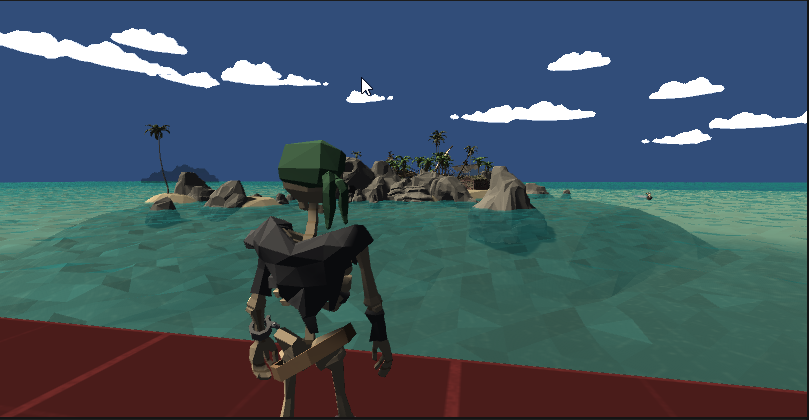
\includegraphics[scale=0.4]{thirdPerson.png}
    \caption{Vue à la troisième personne}
\end{figure}
Pour animer les mouvements des joueurs et des NPC, nous avons utilisé la banque d'animations Mixamo que propose Adobe.
En plus d'avoir des animations détaillées, elles sont entièrement compatible avec le moteur 3D.
\begin{figure}[hbt!]
    \centering
    \begin{subfigure}[b]{0.3\textwidth}
        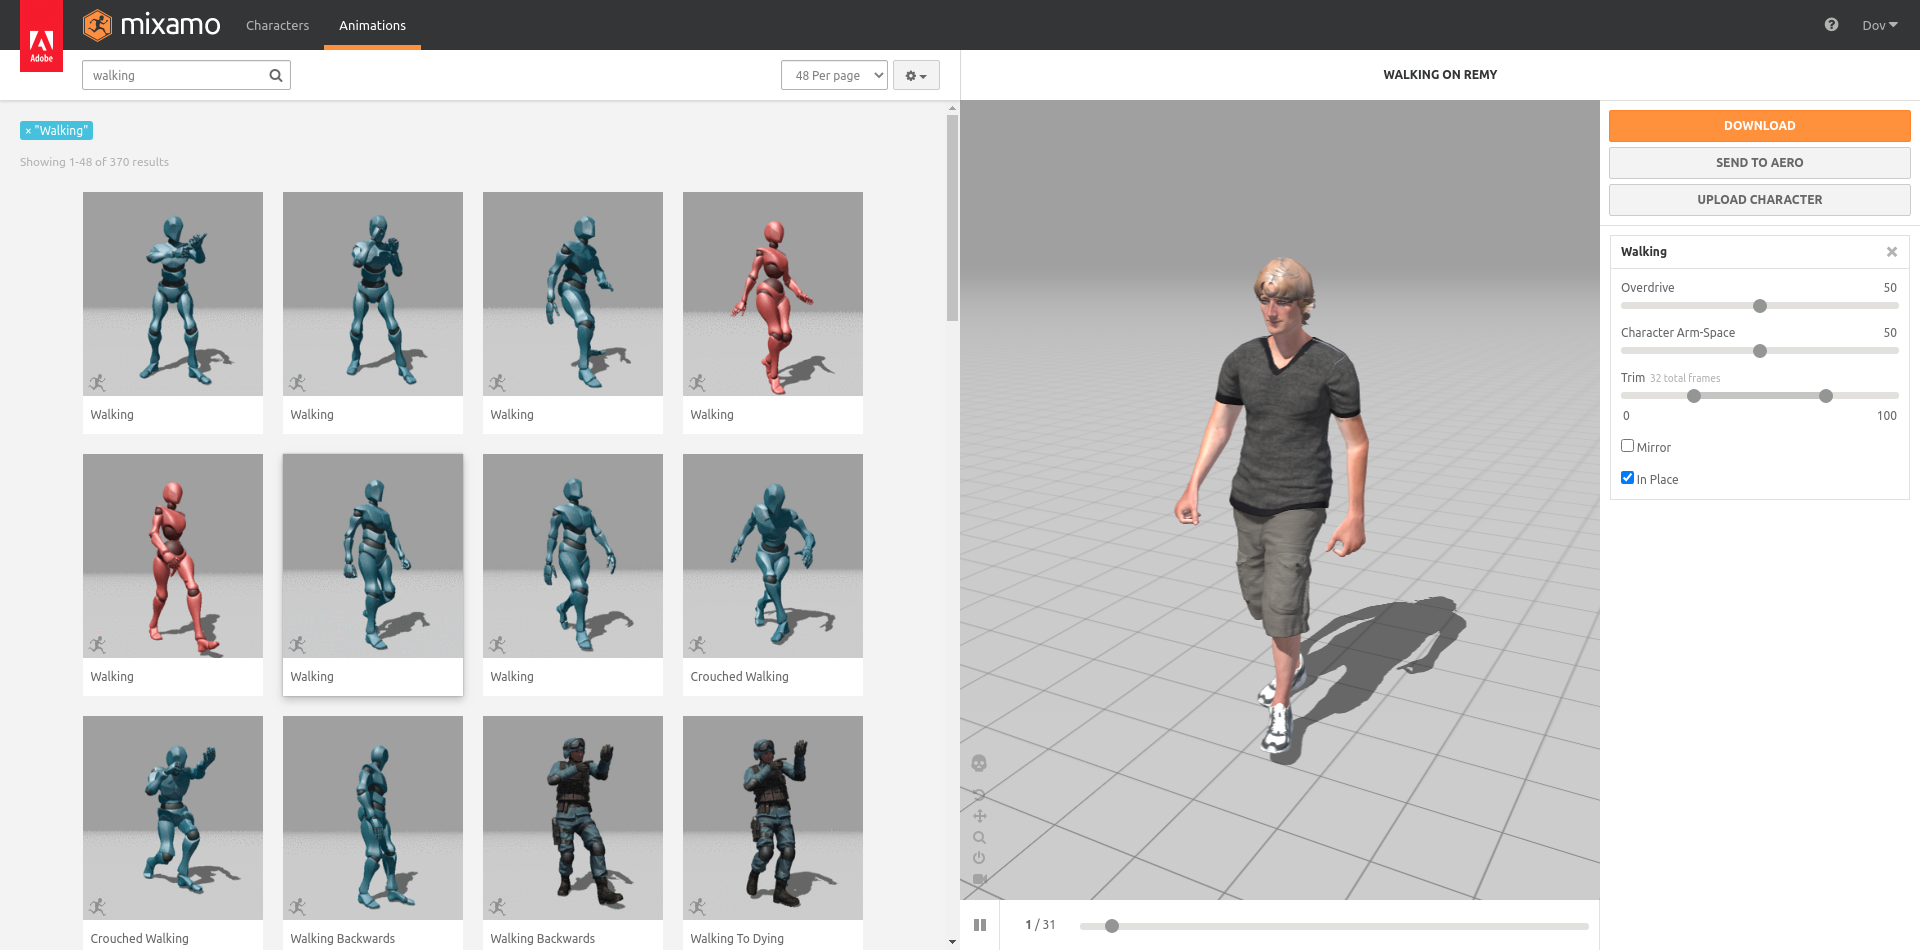
\includegraphics[scale=0.1]{mixamo.png} 
        \caption{Banque d'animations Mixamo}
    \end{subfigure}
    \hfill
    \begin{subfigure}[b]{0.3\textwidth}
        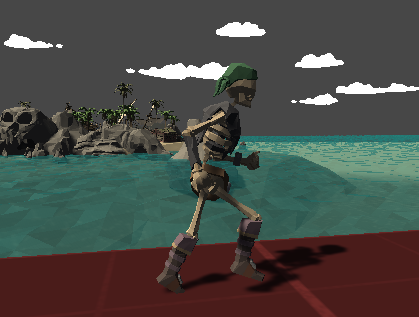
\includegraphics[scale=0.45]{running.png} 
        \caption{Animation de course sur un personnage}
    \end{subfigure}
    \caption{Animations de Mixamo vers Unity}
\end{figure}
% \FloatBarrier



\end{document}